\begin{figure}[htbp]
    \centering
    \adjustbox{valign=t}{ % Adjust first subfigure for top alignment
        \begin{subfigure}{0.47\textwidth}
            \centering
            \adjustbox{valign=t}{
                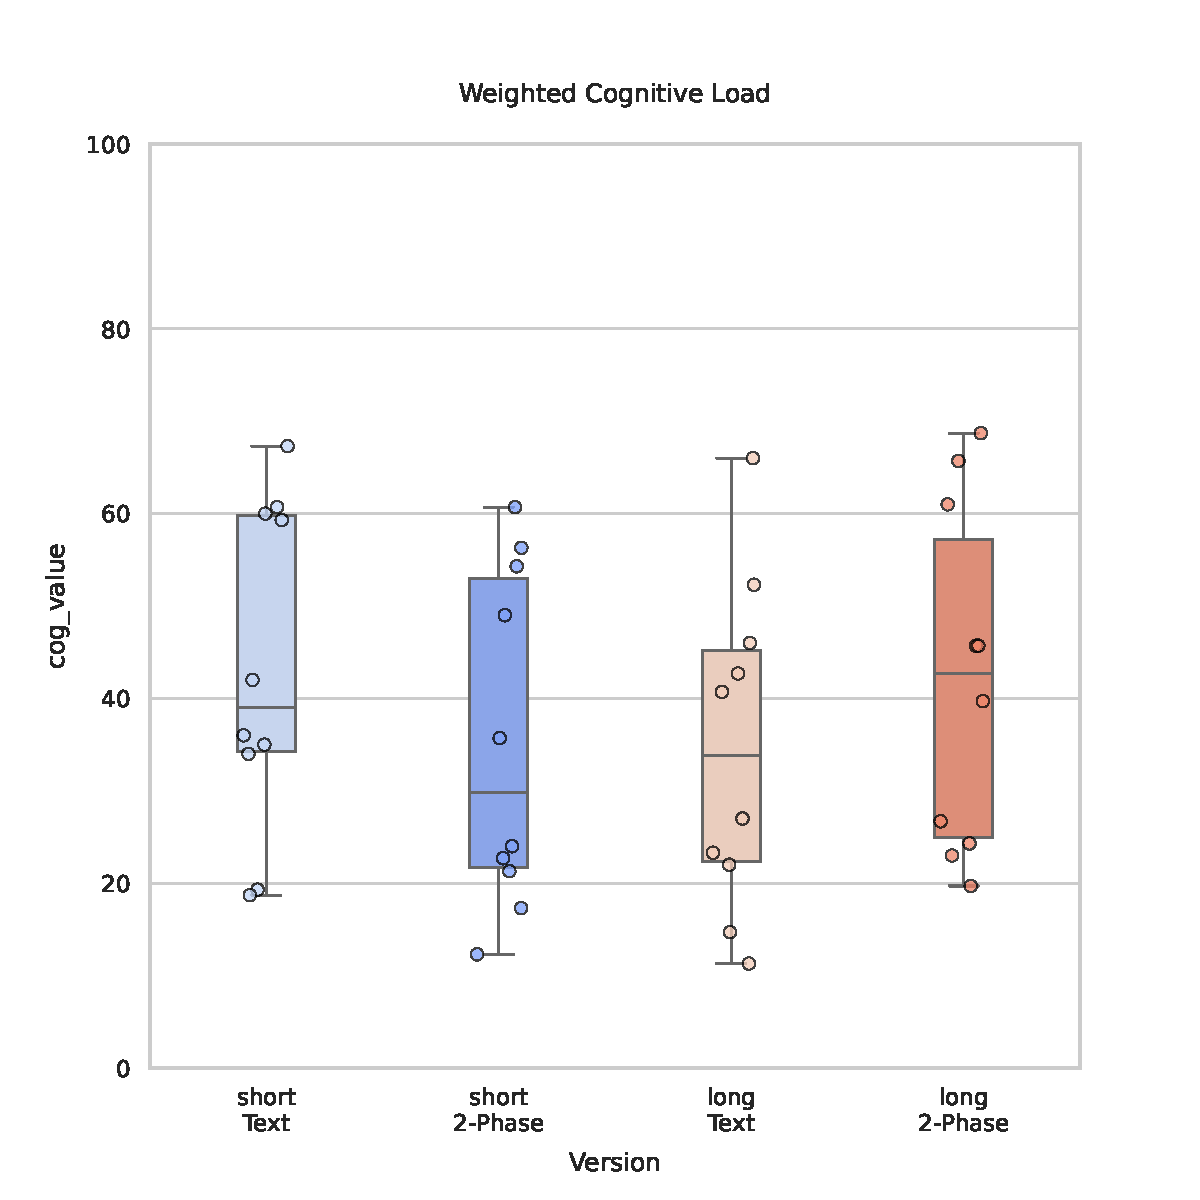
\includegraphics[width=0.95\textwidth]{content/image/results/nasatlx_final_value.pdf}
            }
            \caption{NASA-TLX Weight Score: The Long Two-Phase Interface exhibits the highest weighted cognitive load with a median of $42.70$, a mean of $42.02$. This is higher than the Long Text Interface, which has a median cognitive load of $33.85$ and a mean of $34.60$. However, the Short Text Interface demonstrates a higher cognitive load with a median of $39.00$, a mean of $43.23$, compared to the Short Two-Phase Interface which has a median of $29.85$, a mean of $35.36$. Standard deviation is similar across groups at around $18$.}
            \label{fig:nasatlx-final1}
        \end{subfigure}
    }
    \hfill
    \adjustbox{valign=t}{ % Adjust second subfigure for top alignment
        \begin{subfigure}{0.49\textwidth}
            \centering
            \adjustbox{valign=t}{
                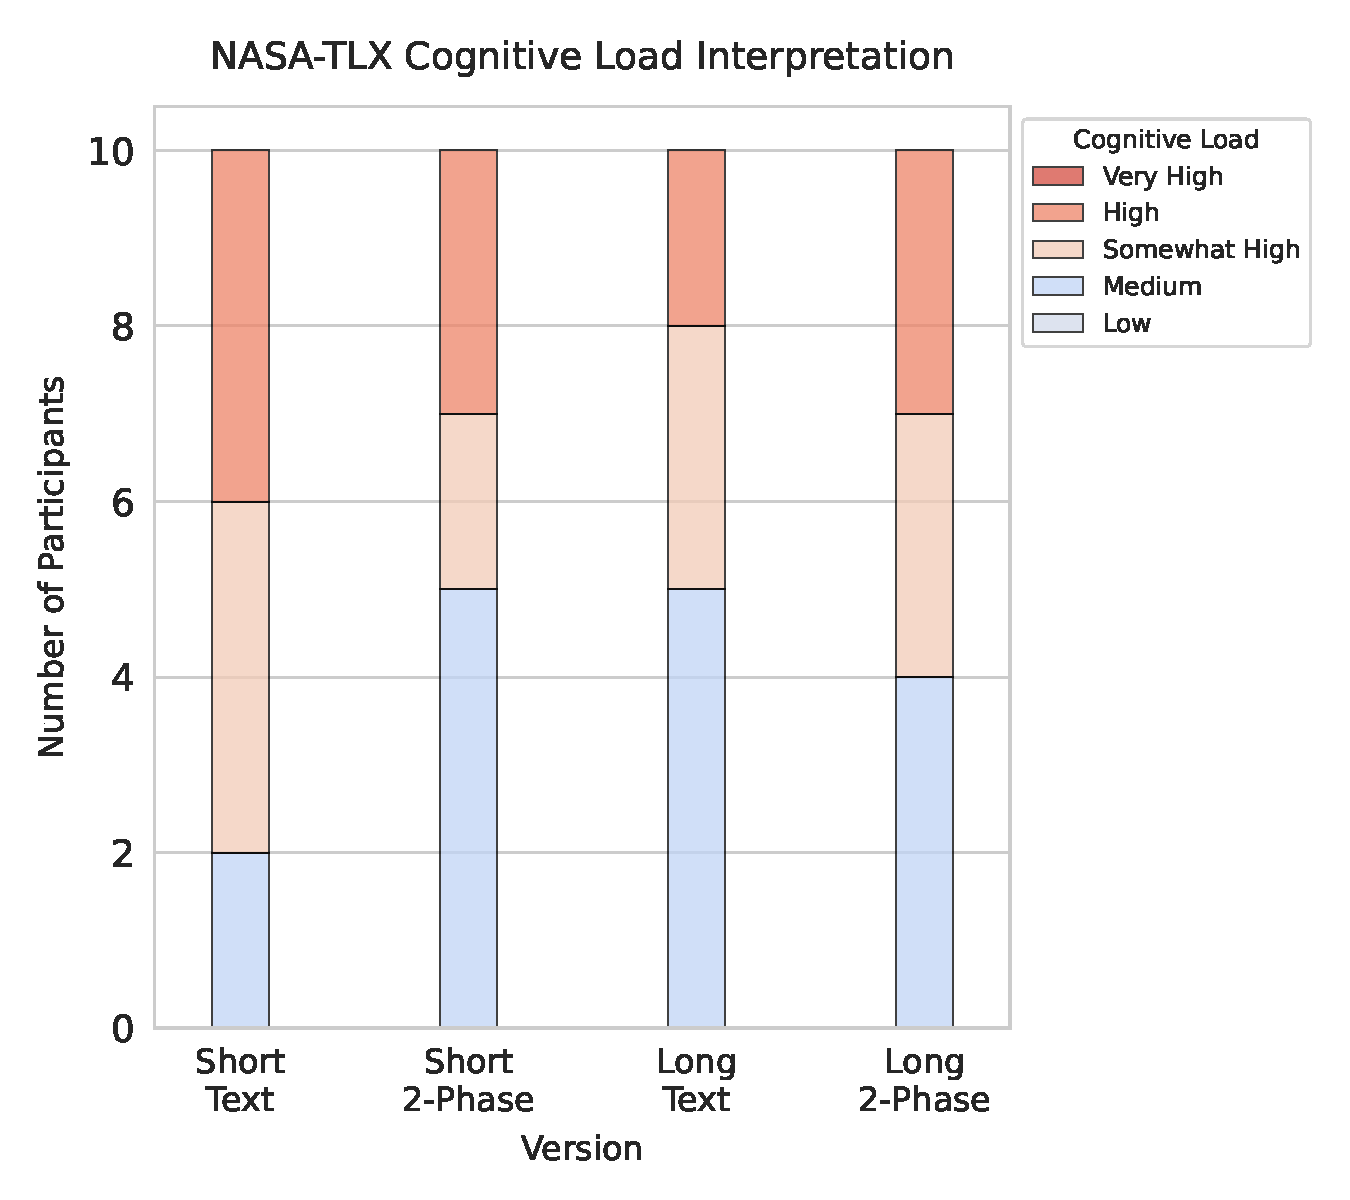
\includegraphics[width=1.05\textwidth]{content/image/results/nasatlx_cog_value_interpreted.pdf}
            }
            \caption{NASA-TLX Cognitive Interpretation: More participants in the Short Text Interface, totaling $8$, reported a somewhat high or above cognitive load, which is significantly higher compared to the $5$ participants who reported similarly for the Short Two-Phase Interface. However, the Long Two-Phase Interface saw slightly more participants, $6$ in total, reporting somewhat high or above cognitive load compared to the Long Text Interface.}
            \label{fig:nasatlx-final2}
        \end{subfigure}
    }
    \caption{This figure shows the box plot results for weighted NASA-TLX scores across experiment groups and participant counts based on individual score interpretations. In~\ref{fig:nasatlx-final1}, we observe a downward trend in cognitive load for the short QS, while the long QS shows an upward trend. Interestingly, there is a counterintuitive downward trend between short and long text interfaces. In~\ref{fig:nasatlx-final2}, these trends are clearer when NASA-TLX scores are grouped into five tiers.}
    \label{fig:nasatlx-final}
\end{figure}


\section{Cognitive Load and Sources across Experiment Conditions}
\label{sec:cog_result}
This section presents cognitive load across experiment groups and the sources contributing to each cognitive load dimension. Due to the smaller sample size, we focus on descriptive statistics and qualitative assessments. We present quantitative data from survey tasks and qualitative insights from post-survey interviews.

The first author conducted an inductive thematic analysis~\cite{olsonWaysKnowingHCI2014} after transcribing the interviews. Snippets were coded based on research questions and topics of interest, and similar codes were merged to form themes. When differences emerged across experiment conditions and hypotheses were formed, the first author applied a deductive coding process to the relevant text snippets. We begin by presenting an overview of the cognitive load findings. 

\subsection{Overall Cognitive Load}
\label{sec:cog}

To answer our research question on how the number of options in QS~(\textbf{RQ1}) and the interface~(\textbf{RQ2a}) impacted cognitive load, we derive the weighted NASA-TLX scores across the four experiment conditions. We show these results in Figure~\ref{fig:nasatlx-final}. Weighted NASA-TLX uses a continuous $0$-$100$ score, with higher values indicating greater cognitive load. We use predefined mappings of NASA-TLX scores to cognitive levels: low, medium, somewhat high, high, and very high, as listed by~\textcite{hart1988development}. We show value interpretations in Figure~\ref{fig:nasatlx-final2}. 
% We provide summary statistics of the scores here as well:

% \begin{itemize}
%     \item Short text interface: The median cognitive load was $39.00$, with a mean of $43.23$ and a standard deviation of $17.65$. $8$ participants reported somewhat high or above, with $4$ reporting high cognitive load.
%     \item Short two-phase interface: The median cognitive load was $29.85$, with a mean of $35.36$ and a standard deviation of $18.17$. $5$ participants reported somewhat high or above, with $3$ reporting high cognitive load.
%     \item Long text interface: The median cognitive load was $33.85$, with a mean of $34.60$ and a standard deviation of $17.69$. $5$ participants reported somewhat high or above, with $2$ reporting high cognitive load.
%     \item Long two-phase interface: The median cognitive load was $42.70$, with a mean of $42.02$ and a standard deviation of $18.48$. $6$ participants reported somewhat high or above, with $3$ reporting high cognitive load.
% \end{itemize}

Surprisingly, the long text interface had lower mean~($\mu=34.60$) and median~($\tilde{x}=33.85$) cognitive load scores than both the short text~($\mu=43.23$, $\tilde{x}=39.00$) and long two-phase interfaces~($\mu=42.02$, $\tilde{x}=42.70$). Additionally, the two-phase interface decreased cognitive load for the short survey but increased it for the long survey. Notably, the short text interface had the most participants~($N=8$) reporting somewhat high or higher cognitive loads. In contrast, the other conditions had a more balanced distribution, with about half reporting medium to high loads.

We acknowledge that these results may not fully reflect actual cognitive load due to potential noise from factors such as small sample size, task nature, or participants' interpretation of the scale. To explore the similarities and sources of cognitive load across interfaces~(\textbf{RQ2b}), we turn to qualitative insights from post-task interviews based on NASA-TLX cognitive load dimensions. Among the six NASA-TLX dimensions, we focus on mental demand, temporal demand, and frustration while summarizing key findings regarding physical demand, performance, and effort for brevity. Appendix~\ref{apdx:cog_qual} provides further details on all six dimensions.

% ============================================= %
\subsection{Sources of Mental Demand}
\label{sec:mental}
We began by examining mental demand, which refers to the amount of mental and perceptual activity required to complete a task. Interview results indicated that the primary drivers of participants' mental demand were~\textit{Budget management} and~\textit{Preference construction}.

\subsubsection{Mental Demand Source \#1: Budget management} $14$ participants expressed demand from budgeting within limited credit~(\smallquote{S032}{~\bracketellipsis for certain societal issues you had to~\ldots take away from other societal issues that you could support.}, $N=5$), tracking remaining credits~(\smallquote{S006}{~\bracketellipsis looking at the remaining credits, I'm trying to mentally divide that up before I start allocating}, $N=10$), and maximizing credit use~(\smallquote{S032}{~\bracketellipsis I used all the credit that I had available}, $N=8$).

We categorized budget management-induced mental demand as either operational~(single interface-level action, e.g., using the last remaining credit) or strategic~(higher-level goal, e.g., evenly distributing credits across options). Participants who completed longer surveys more frequently reported operational causes, suggesting that an increase in survey options induced short-term thinking.

\subsubsection{Mental Demand Source \#2: Preference construction}
All but one participant reported increased mental demand due to preference construction. We further break it down into three sources: comparative preference evaluation~(i.e., evaluating relative importance between options; \smallquote{S002}{Figuring out \dots how much I prioritize option 1 over option 2}, $N=16$), resource-constraint prioritization~(i.e., trading off between options due to resource constraints, \smallquote{S005}{~\bracketellipsis very hard to take decisions~\ldots because I felt that multiple options deserve equal amount of credit~\ldots but you have given very limited amount of credit.}, $N=17$), and deciding the exact number of votes~(\smallquote{S023}{~\bracketellipsis having to pick how many upvotes would go to each one}, $N=30$).

Almost all participants mentioned preference construction as a source of mental demand, supporting our claim that preference construction when completing QS is a difficult and mentally demanding task. Notably, more participants using the text interface reported mental demand from deciding the exact number of votes compared to the two-phase interface~($18$ vs. $12$). We conjecture that the first pass on the survey items and organizing them helped participants construct preliminary preferences and reduced their mental demands when they started allocating votes.

In addition, when categorizing preference construction-induced mental demand, participants~($N=8$) in the long text interface tend to consider a smaller scope that focuses on personal relevance. Conversely, participants~($N=9$) in the long two-phase interface considered the broader societal impact and evaluated options more comprehensively. Compare the following two quotes, where one focused on adjusting credits between two options and the other reflecting across broader societal values:

\begin{displayquote}
Trying to figure out what upvotes I should give~\bracketellipsis went back and forth between those two. \bracketellipsis it was very mentally tasking for me. \hfill\quoteby{S015~(LT)}
\end{displayquote}

\begin{displayquote}
\bracketellipsis really having to think, especially with so many different societal issues. How do I personally prioritize them? And to what extent do I prioritize them? \hfill\quoteby{S009~(LI)}
\end{displayquote}

Inspecting both causes, we did not notice significant differences in mental demand raw values~(Figure~\ref{fig:mental_cog_score}) across the four experiment groups, especially between the interfaces across long QS. However, the experiment groups' mental demands came from different sources.

% Discussion: We argue the two-phase interface prevented participants from using heuristics to narrow their choices, which only appeared when final votes were determined, an area with less support from the interface. We conclude the two-phase interface scaffolded the decision-making process, preventing satisficing behaviors because of cognitive overload, and thus shifted mental demand sources. This shift explains why .

% ============================================= %

% \begin{wrapfigure}{r}{0.45\textwidth} % Adjust the width as needed
%    \centering
%     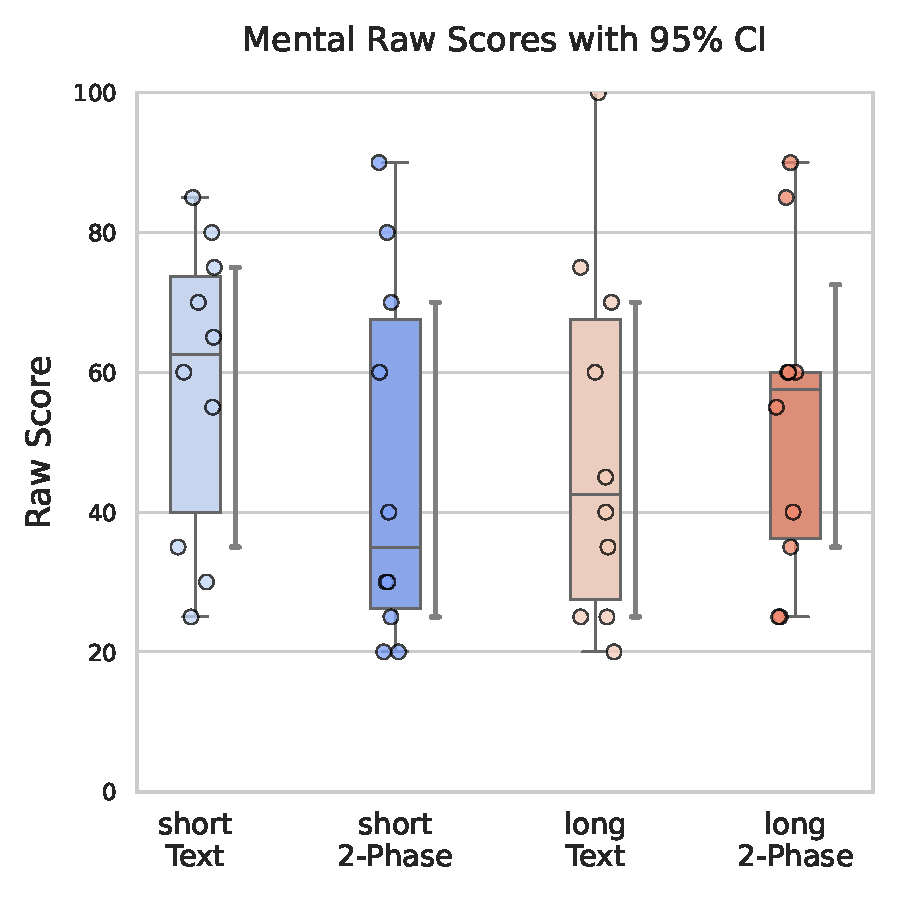
\includegraphics[width=0.45\textwidth, trim=0 13 0 13, clip]{content/image/cog/Mental_scores.pdf}
%     \captionsetup{width=0.4\textwidth, justification=justified}
%     \caption{Mental Demand Raw Score: Across all four experiment groups, participants' reported mental demand is spread across a wide range with many participants experiencing high mental demand.}
%     \label{fig:mental_cog_score}
% \end{wrapfigure}

% \begin{wrapfigure}{r}{0.45\textwidth} % Adjust the width as needed
%     \centering
%     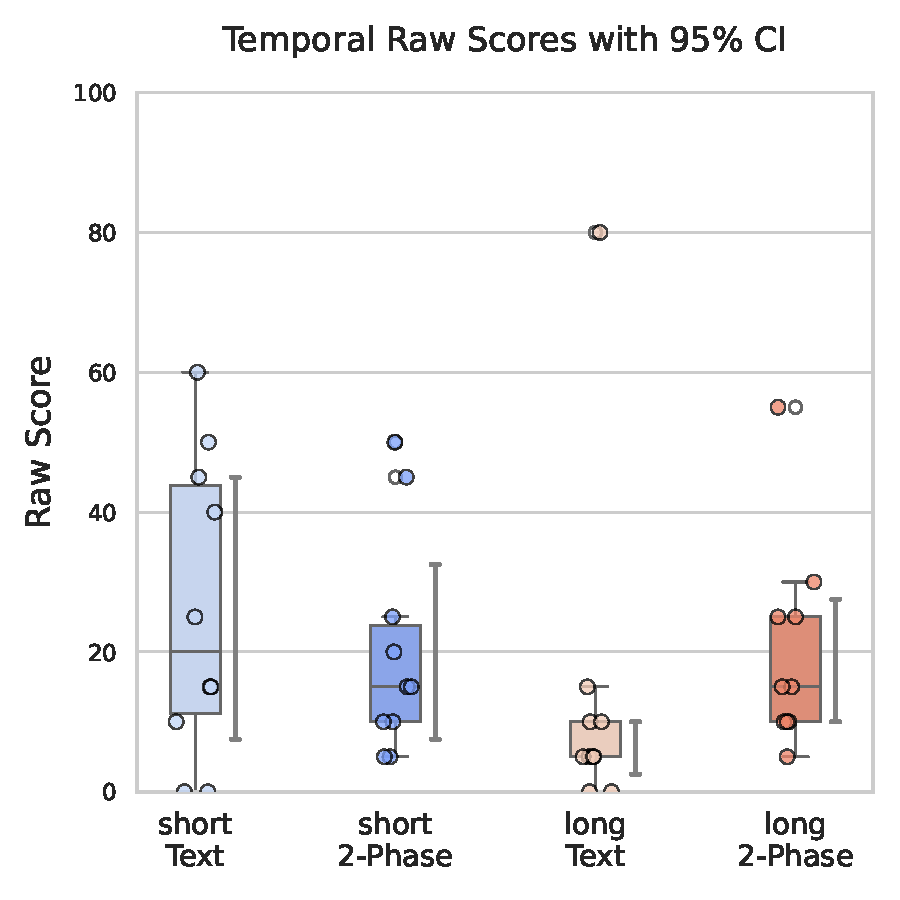
\includegraphics[width=0.45\textwidth, trim=0 13 0 13, clip]{content/image/cog/Temporal_scores.pdf}
%     \captionsetup{width=0.45\textwidth, justification=justified} % Adjust the width to match the image width
%     \caption{Temporal Demand Raw Score: The short text interface results in the highest temporal demand, while the long text interface is the lowest. Two-phase interfaces, show moderate temporal demand, suggesting that interactive elements allowed participants to pace themselves better.}
%     \label{fig:temporal_cog_score}
% \end{wrapfigure}

\begin{figure}[t!]
    \centering
    % First figure and caption
    \adjustbox{valign=t}{
        \begin{minipage}{0.48\textwidth} % Adjusted width for the first figure
            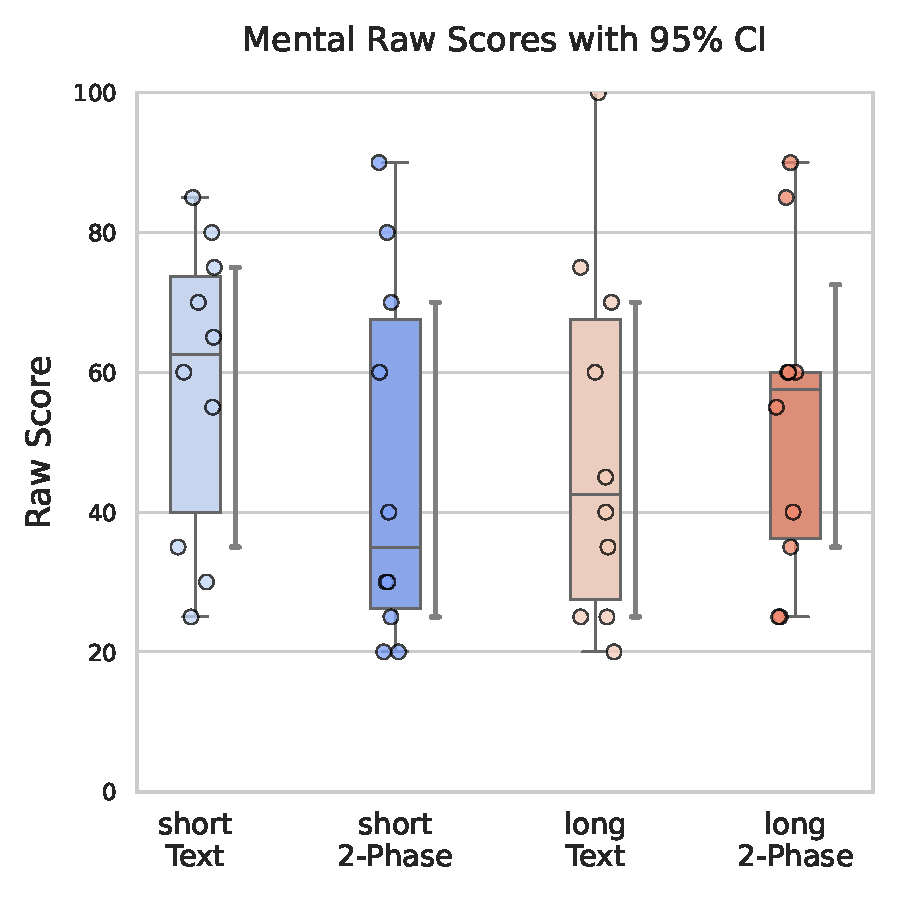
\includegraphics[width=\textwidth, trim=0 13 0 13, clip]{content/image/cog/Mental_scores.pdf}
        \end{minipage}
    }%%%
    \hfill  
    % Second figure and caption
    \adjustbox{valign=t}{
        \begin{minipage}{0.48\textwidth} % Adjusted width for the second figure
            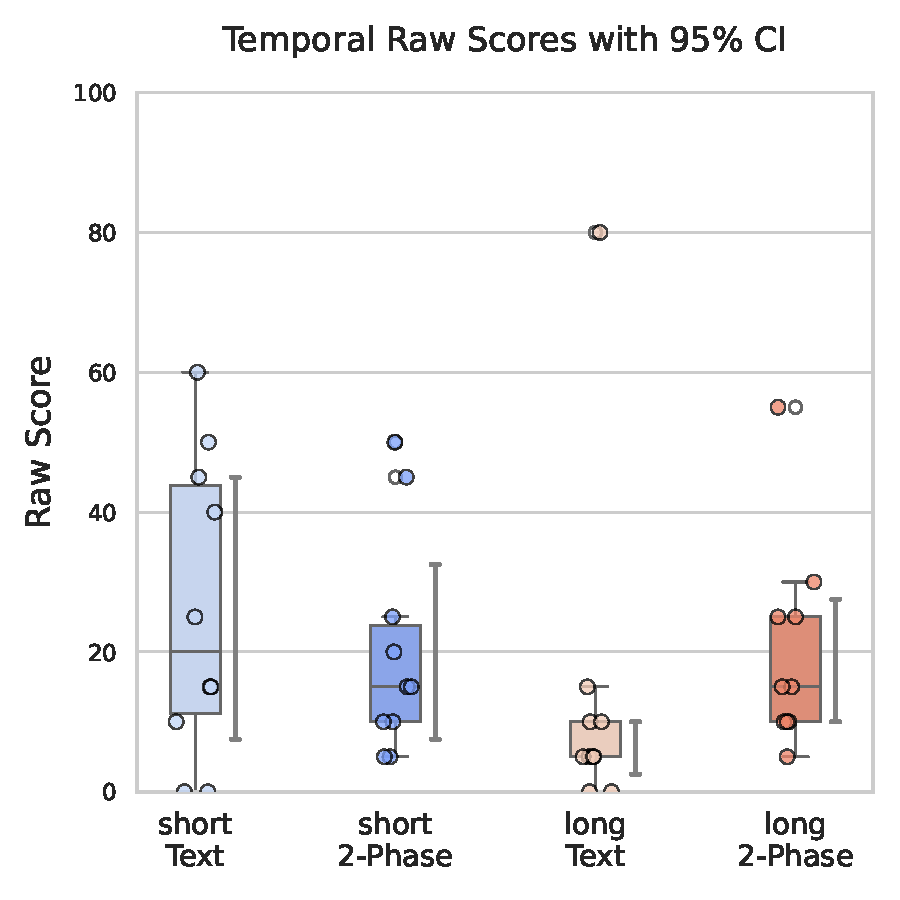
\includegraphics[width=\textwidth, trim=0 13 0 13, clip]{content/image/cog/Temporal_scores.pdf}
            \vfill
        \end{minipage}
    } 
    % First caption
    \begin{minipage}[t]{0.48\textwidth}
        \caption{Mental Demand Raw Score: Across all four experiment groups, participants' reported mental demand is spread across a wide range with many participants experiencing high mental demand.}
        \label{fig:mental_cog_score}
    \end{minipage}%%%
    \hfill
    % Second caption
    \begin{minipage}[t]{0.48\textwidth}
        \caption{Temporal Demand Raw Score: The short text interface results in the highest temporal demand, while the long text interface is the lowest. Two-phase interfaces show moderate temporal demand, suggesting that interactive elements allowed participants to pace themselves better.}
        \label{fig:temporal_cog_score}
    \end{minipage}
\end{figure}


% ============================================= %

\subsection{Sources of Temporal Demand} 
\label{sec:temporal}

Temporal demand measures the time pressure participants feel during a task. Lower demand indicates participants taking a more leisurely pace. The main sources of increased temporal demand relate to time pressure on ~\textit{Decision-Making}~(\smallquote{S024}{maybe I should just hurry up and make a decision.}, $N=15$) and ~\textit{Operational Tasks}~(\smallquote{S032}{to be able to move through this quickly and efficiently}, $N=16$)~(Table~\ref{tbl:temporal}). Additionally, some participants mention~\textit{Budget management} as a source of temporal demand~(\smallquote{S034}{as the money decreases I felt kind of rushed}, $N=4$).

\subsubsection{Two-phase Interface Reduced Temporal Demand on Short QS} The raw NASA-TLX values in Fig~\ref{fig:temporal_cog_score} show that participants in the Short Text Interface reported the highest temporal demand. Five participants expressed concerns about time spent on decision-making, feeling themselves invested more time and effort than expected, prompting them to rush. However, the two-phase interface reduced this, with only one participant in the short survey group reporting similar concerns.

\subsubsection{Long QS on Text Interface Showed the Lowest Temporal Demand} 
Surprisingly, participants in the long text interface exhibited the lowest temporal demand~(Fig.~\ref{fig:temporal_cog_score}) despite making more decisions and operations compared to the short text group. Two possible explanations might explain this counter-intuitive result. First, more participants in the short survey group ($N=7$) expressed a desire to complete the task efficiently, compared to just one participant ($N=1$) in the long survey group, saying things like:

\begin{displayquote}
I wanna get through things in an efficient manner~\bracketellipsis to move through this quickly and efficiently. \hfill\quoteby{S032~(ST)}
\end{displayquote}
% which doesn't necessarily mean I rush it. But it does mean that I do things expeditiously. Especially. I'd like to think I'm somewhat computer-savvy. And so to be able
% I do take pride in it, but it's all personal stuff. It's not nothing outwardly influencing me. 

Second, satisficing behaviors may explain the lower temporal demand in the long text condition. Participants may have experienced cognitive overload from the long list of options and, as a result, spent less time than expected on decisions. For example:
\begin{displayquote}
I didn't really do the math, so I was like \$2 is not that much left so I tried my best to use up most of it. \\\hfill\quoteby{S035~(LT)}
\end{displayquote}

We will discuss this possibility further in Section~\ref{sec:satisficing}.

\subsubsection{Two-phase Interface Increased Temporal Demand in Long QS} Despite the unexpectedly low temporal demand in long QS with a text interface, two-phase interface participants have indifferent temporal demand across survey lengths. All five participants who mentioned a feeling of time pressure on decision-making in the long two-phase group described the pressure affirmatively. This means their pressure stemmed from having too many remaining decisions to make~(\smallquote{S022}{So it didn't take too much time. but obviously there were a lot of things to consider, so there was some temporal demand.}), not from the time they have already spent~(i.e., framed negatively) as that in the short text group. 

% \subsubsection{Temporal Demand Source \#1: Decision Making}
% Participants often felt there were too many decisions to make. We observe no significant difference in how often participants expressed concerns about temporal demand across conditions. However, how they expressed their concerns differed. These concerns were either expressed affirmatively or negatively. Affirmative expression refers to cases where participants stated there were too many remaining decisions to make~(\smallquote{S022}{So it didn't take too much time. but obviously there was a lot of things to consider, so there was some temporal demand.}), while negative expression refers to participants' concerns regarding the time and effort already invested~(\smallquote{S024}{maybe I should just hurry up and make a decision.}). Five participants from the short text interface expressed negative perceptions of temporal demand and no participants expressed concerns affirmatively. In contrast, five participants from the long two-phase interface expressed affirmatively with zero negatively.

% \subsubsection{Temporal Demand Source \#2: Operational Tasks}
% Lower-level operational tasks were also often discussed as sources of temporal demand. Operational tasks involve actions like updating votes and completing the survey. For instance, one participant aimed to operate swiftly:

% \begin{displayquote}
% I wanna get through things in an efficient manner which doesn't necessarily mean I rush it. But it does mean that I do things expeditiously. Especially. I'd like to think I'm somewhat computer-savvy. And so to be able to move through this quickly and efficiently. I do take pride in it, but it's all personal stuff. It's not nothing outwardly influencing me. \hfill\quoteby{S032~(ST)}
% \end{displayquote}

% The raw NASA-TLX values in Fig~\ref{fig:temporal_cog_score} first highlighted that temporal demand trended lower for the two-phase interface in the short QS condition while it trended higher for the long QS condition. Second, the long text interface exhibited the lowest temporal demand, which is counter intuitive since participants in this condition made no fewer decisions and operations compared to the short text group. Although we were initially surprised to find that temporal demand was higher for the short survey experiment group, we noticed that more participants who experienced a short survey expressed a desire to complete the task quickly. Over half of the participants from the short interface wanted to complete the task swiftly and quickly, compared to $5$ participants from the long QS group. Thus, our counter-intuitive findings around temporal demand may be explained by the fact that participants who received the short survey had higher expectations to complete the survey swiftly.

%\subsubsection{Takeaway: Temporal demand managed through two-phase interface}
%The raw NASA-TLX values in Fig~\ref{fig:temporal_cog_score} visually indicate two important points. First, temporal demand trended lower for the two-phase interface in the short QS condition, while it trended higher for the long QS condition. Second, the long text interface exhibited the lowest temporal demand, which is counterintuitive since participants in this condition made no fewer decisions and operations compared to the short text group. According to our interpretation of mental demand results in Section~\ref{sec:mental_takeaway}, participants likely did not experience temporal demand because they applied heuristics to reduce the number of decisions, thereby lowering their cognitive load and decision-making instances.

%Additionally, participants in the long interactive condition reported that the numerous required operations created temporal demand, preventing them from taking mental shortcuts and shifting their cognitive load to different dimensions.

%Furthermore, participants in the short text QS expressed high temporal demand and perceived it negatively, likely misperceiving task difficulty. Conversely, even though the short two-phase interface required more decisions, participants reported less temporal demand from decision-making, resulting in a lower overall score. This suggests that the two-phase interface slowed them down without increasing temporal demand, allowing them to pace themselves and engage in more in-depth thinking, thereby preventing a misperception of task difficulty.

%These observations across experimental conditions support the plausible explanation that the two-phase interface mitigated satisficing behaviors due to cognitive overload, as evidenced by the different sources of temporal demand.

%  TODO: move to discussion?
% It is also worth noting that three participants from the 20 who responded to the long survey mentioned that the vertical screen's ability to see all options facilitated direct comparisons and transparency about the entirety of the task, which reduced the temporal demand.

% \begin{displayquote}
%~(Seeing) all at once I can see how many there are, so it's kind of like I can kind of tell when I will be done.

% \noindent \hfill -- S041, long text interface
% \end{displayquote}

%
% ============================================= %

\subsection{Source of Frustration} 
\label{sec:frustration}

Frustration refers to the extent to which the participant is annoyed, irritated, or discouraged during the task. We identified either \textit{Operational Actions}~(e.g., credit management~($N=6$) and managing quadratic vote costs~($N=5$)), or \textit{Societal Concerns}~(e.g., regretful trade-offs~($N=8$) or pessimism about other's vote~($N=6$)) as sources of frustration.

In general, the frustration derived from societal concerns did not seem strongly affected by any of the experimental conditions. We saw some discrepancies with respect to operational action-driven frustration. The long text interface condition had the fewest participants expressing operational frustration, with half expressing no frustration, mirroring the trends in the actual scores~(Figure~\ref{fig:frustration_cog_score}). Similar to the finding that the long text group has the lowest temporal demand, this is counter-intuitive as more options and dense text are known to lead to more frustration in interface design~\cite{nielsen1997users}. Participants engaging in satisficing behaviors in the long text interface may explain this phenomenon -- prior literature~\cite{polmanWhyAreMaximizers2010, schwartzMaximizingSatisficingHappiness2002} indicates that satisficers tend to be less frustrated and happier than maximizers. 

\begin{wrapfigure}{r}{0.45\textwidth} % Wrap figure on the right
    \centering
    \adjustbox{valign=t}{
        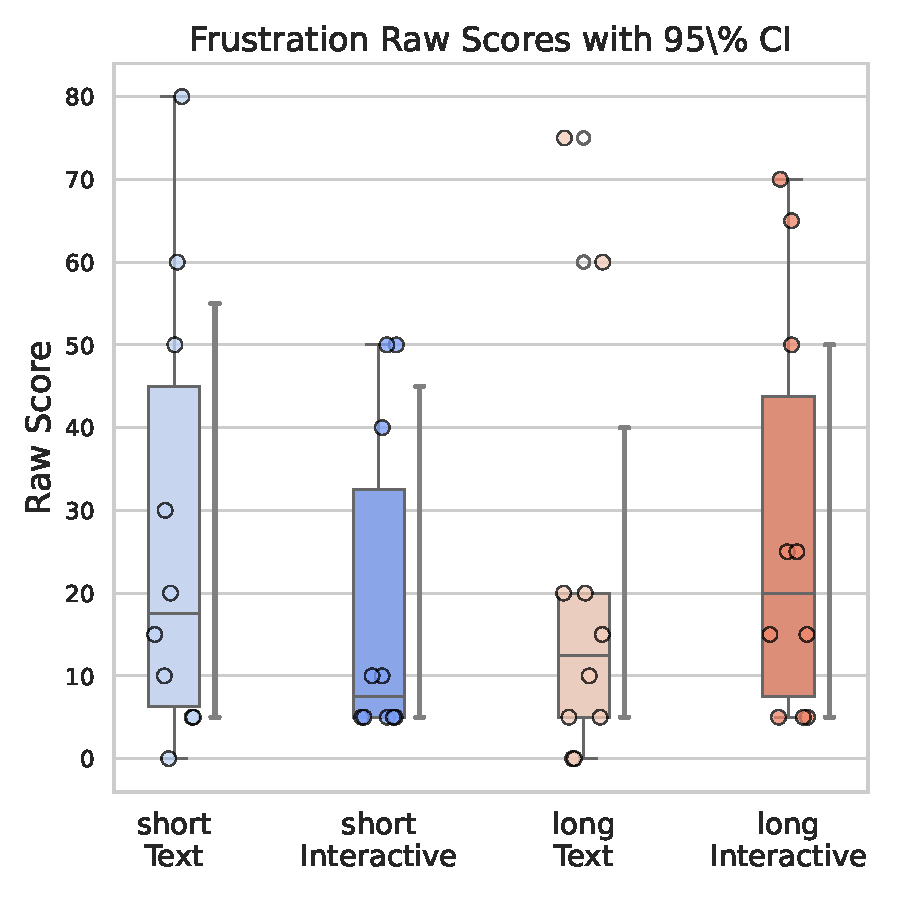
\includegraphics[width=\linewidth, trim=0 13 0 13, clip]{content/image/cog/Frustration_scores.pdf}
    }
    \captionsetup{width=0.9\linewidth, justification=justified}
    \caption{Frustration Raw Score: Participants other than the long text interface highlighted several operational tasks that led to frustration. All groups share causes from strategic planning.}
    \label{fig:frustration_cog_score}
\end{wrapfigure}

%\subsubsection{Operational Actions} 
%$15$ participants highlighted this source for frustration. $6$ participants expressed frustration regarding credit management~(i.e., overspending budget); $4$ participants mentioned had trouble deciding the final value for the options; $3$ participants are frustrated because they need to make multiple decisions; $5$ participants were frustrated with the quadratic mechanism; $4$ participants are frustrated trying to understand the content of the option or how the option connects to them. For example, 

%\begin{displayquote}
%I was slightly frustrated when doing the task, probably because there was a budget that we kind of had to stick with it.

%\noindent \hfill -- S001, long text interface, quadratic mechanism
%\end{displayquote}

%\begin{displayquote}
%i think just frustration~\bracketellipsis because when i was making like the decisions on how many upvotes I could put in each section, I was running out of credits.

%\noindent \hfill -- S013, short two-phase interface, budget management
%\end{displayquote}

%These demonstrate participants' frustration when hindered by operational actions or constraints presented by QS. Notably, almost half of the participants in all experiment groups expressed operational frustration, compared to only two participants from the long text interface group.

%\begin{wrapfigure}{r}{0.45\textwidth} % Adjust the width as needed
%    \centering
 %   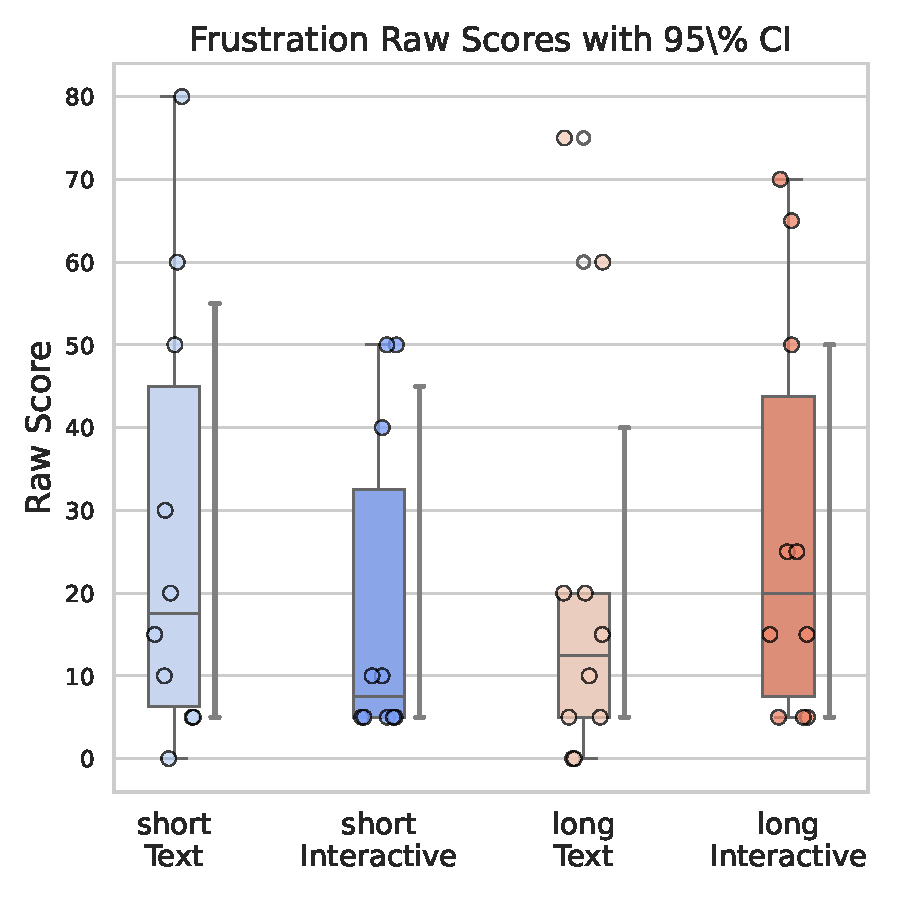
\includegraphics[width=0.45\textwidth, trim=0 13 0 13, clip]{content/image/cog/Frustration_scores.pdf}
 %   \captionsetup{width=0.40\textwidth, justification=justified} % Adjust the width to match the image width
  %  \caption{Fustration Raw Score: Participants other than the long text interface highlighted seversl operational tasks that led to fustration. All groups share causes from strategic planning.}
    %\label{fig:fustration_cog_score}
%\end{wrapfigure}

%\subsubsection{Strategic Planning}
%We derived strategic planning into two types: \textit{lower-level} and \textit{higher-level}. Four participants experienced conflict between their own and others' preferences. Eight participants experienced conflict when making trade-offs among a few options. For example:

%\begin{displayquote}
%Because I know that's important to other people. But it just doesn't to me.
    
%\noindent \hfill -- S010, short two-phase interface
%\end{displayquote}

%\begin{displayquote}
%I would have loved to have given more to other groups~\ldots and I felt stressed like~\bracketellipsis well~\ldots it's a group that you know is still~\ldots you know~\ldots important~\bracketellipsis
%\noindent \hfill -- S020, long text interface
%\end{displayquote}

%These quotes show participants adhering to lower-level strategies like balancing personal preferences and smaller trade-offs. Compared to~\textit{higher-level strategic planning}, $6$ participants expressed conflicts involving broader societal concerns and core values. $8$ participants felt frustrated by being forced to make trade-offs among~\textit{all} options. For example,

%\begin{displayquote}
%I had to consider how I feel towards that~\ldots how religious media broadcasting is being used in like today's society~\ldots today's political environment. So yeah~\ldots you really have to consider what is important to you. 
%\noindent \hfill -- S020, long text interface, value conflicts
%\end{displayquote}

%\begin{displayquote}
%I think the frustration is~\ldots I wish that we could help all of these causes, but you know it's just like anything else. You can't do everything and when it's not~\ldots  I feel like it's hard to quantify how much some of these things should be supported versus others. So when you're talking about upvotes and things that's challenging to me, it's frustrating.
%\noindent \hfill -- S026, long two-phase interface, considering all options
%\end{displayquote}

%All experimental conditions noted similar frustration related to strategy planning, across lower-level and higher-level frustration.


%============================================= %
\subsection{Physical Demand, Effort and Performance}
Physical demand refers to the physical effort required to complete a task, such as physical exertion or movement. The two-phase interface experienced higher physical demand from increased mouse usage.

Effort refers to how hard participants felt they worked to achieve the level of performance they did. Qualitative analysis showed participants using the two-phase interface, regardless of length, considered options more comprehensively and felt less effort in completing operational tasks. Almost all participants~($N=9$) from the long two-phase interface spent effort planning a strategy to complete tasks with many~($N=7$) considered options comprehensively and beyond the immediate task (i.e., considering the broader community impact of their choices). 

Performance refers to a person's perception of their success in completing a task. An interesting element that contributed to their cognitive load comes from concerning social responsibility. They wonder how their final vote counts would be perceived by others~(\smallquote{S041}{I don't want people to think that I just like don't care about <ethnicity> people at all}) or influence real-world decision-making~(\smallquote{S027}{Some of these things might \ldots have outcomes that I didn't foresee}). In addition, when analyzing how participants describe their performance, we categorize them into indications of satisficing behaviors(``good enough''), exhausting their effort (i.e., ``done their best,''), or feeling positive (i.e., "feeling good.") We observed twice as many participants using the two-phase interface to report the positive feeling about their final submission~($N=11$ v.s. $N=6$).

%============================================= %
\subsection{Summary across all cognitive load dimensions}
Overall, participants using the two-phase interface tend to think more comprehensively and critically, while those using the text interface focus more narrowly on operational tasks. Specifically, we identified that more participants using the text interface reported~\textit{mental demand} from precisely determining the number of votes for options compared to the two-phase interface; and reversely participants using the long two-phase interface considered broader societal impacts and evaluated options holistically. Further, participants using the short text interface wanted to complete the task quickly and reported the highest ~\textit{temporal demand}, compared to participants using the long text interface experienced the lowest. Coupled with our observation participants in the long text interface showed the least amount of~\textit{frustration} from operational causes compared to other experiment conditions. Thus, we suspect that participants who completed the long QS on a text interface engaged in satisficing behaviors based on the counter-intuitive results that they had the lowest temporal demand and frustration level. We will interpret these results in the discussion section. To better understand participants' behavior, we analyze click-stream data across experiment conditions in the next section.

% \begin{itemize}
%     \item \textbf{Mental Demand:} Participants using the text interface reported higher mental demand from determining the number of votes for options. Those using the long two-phase interface considered broader societal impacts and evaluated options holistically.
%     \item \textbf{Physical Demand:} Physical demand was higher for participants using the two-phase interface due to increased mouse usage.
%     \item \textbf{Effort:} Effort sources varied, with text interface participants focusing more on operational tasks, and two-phase interface participants engaging more in strategic planning, reflecting deeper, more comprehensive consideration of options.
%     \item \textbf{Temporal Demand:} Temporal demand was highest in the short text interface, where participants aimed to complete tasks quickly, while the long text interface showed the lowest temporal demand.
%     \item \textbf{Frustration:} Frustration levels from operational causes were lowest in the long text interface.
%     \item \textbf{Performance:} Participants using the two-phase interface felt more positive about their performance, being twice as likely to report "feeling good" about their results compared to the text interface users.
% \end{itemize}



% % Key boxes ================================================================

% %\vspace{5pt}
% \begin{tldrbox} % mental demand summary
%    \faKey~\textbf{Key Differences:} First, slightly more participants using the text interface reported mental demand from precisely determining the number of votes for options compared to the two-phase interface. Second, when it comes to long QS, participants using the long two-phase interface considered broader societal impacts and evaluated options holistically, while those in the long text interface focused on personal relevance and individual issues. % These differences indicate that the two-phase interface encouraged deeper thinking, shifting the source of mental demand. % We find evidence that the two-phase interface prevented cognitive overload.
% \end{tldrbox}


% \begin{tldrbox}%temporal box
%    \faKey~\textbf{Key Differences:} % Participants faced increased temporal demand from: \textit{Budget}, \textit{Decision Complexity}, and \textit{Operational Tasks}. The two-phase interface managed temporal demand more effectively, allowing participants to pace themselves and avoid misperceiving task difficulty.
%     First, participants using the short text interface wanted to complete the task quickly and reported the highest temporal demand. The two-phase interface lowered the temporal demand for short QS. Second, participants using the long text interface showed the lowest temporal demand score. The two-phase interface increased the temporal demand for long QS.
% \end{tldrbox}


% %\vspace{5pt}
% \begin{tldrbox}% frustration box
%    \faKey~\textbf{Key differences:} We observed evidence that participants in the long text interface showed the least amount of frustration from operational causes compared to other experiment conditions.%Participants experienced frustration from two main sources: \textit{Operational Actions} and \textit{Strategic Planning}. We observed evidence that participants in the long text interface showed little frustration, specifically from operational sources, indicating satisficing behaviors.
% \end{tldrbox}

% ==========================================================================



% \begin{figure}[ht]
%     \centering
%     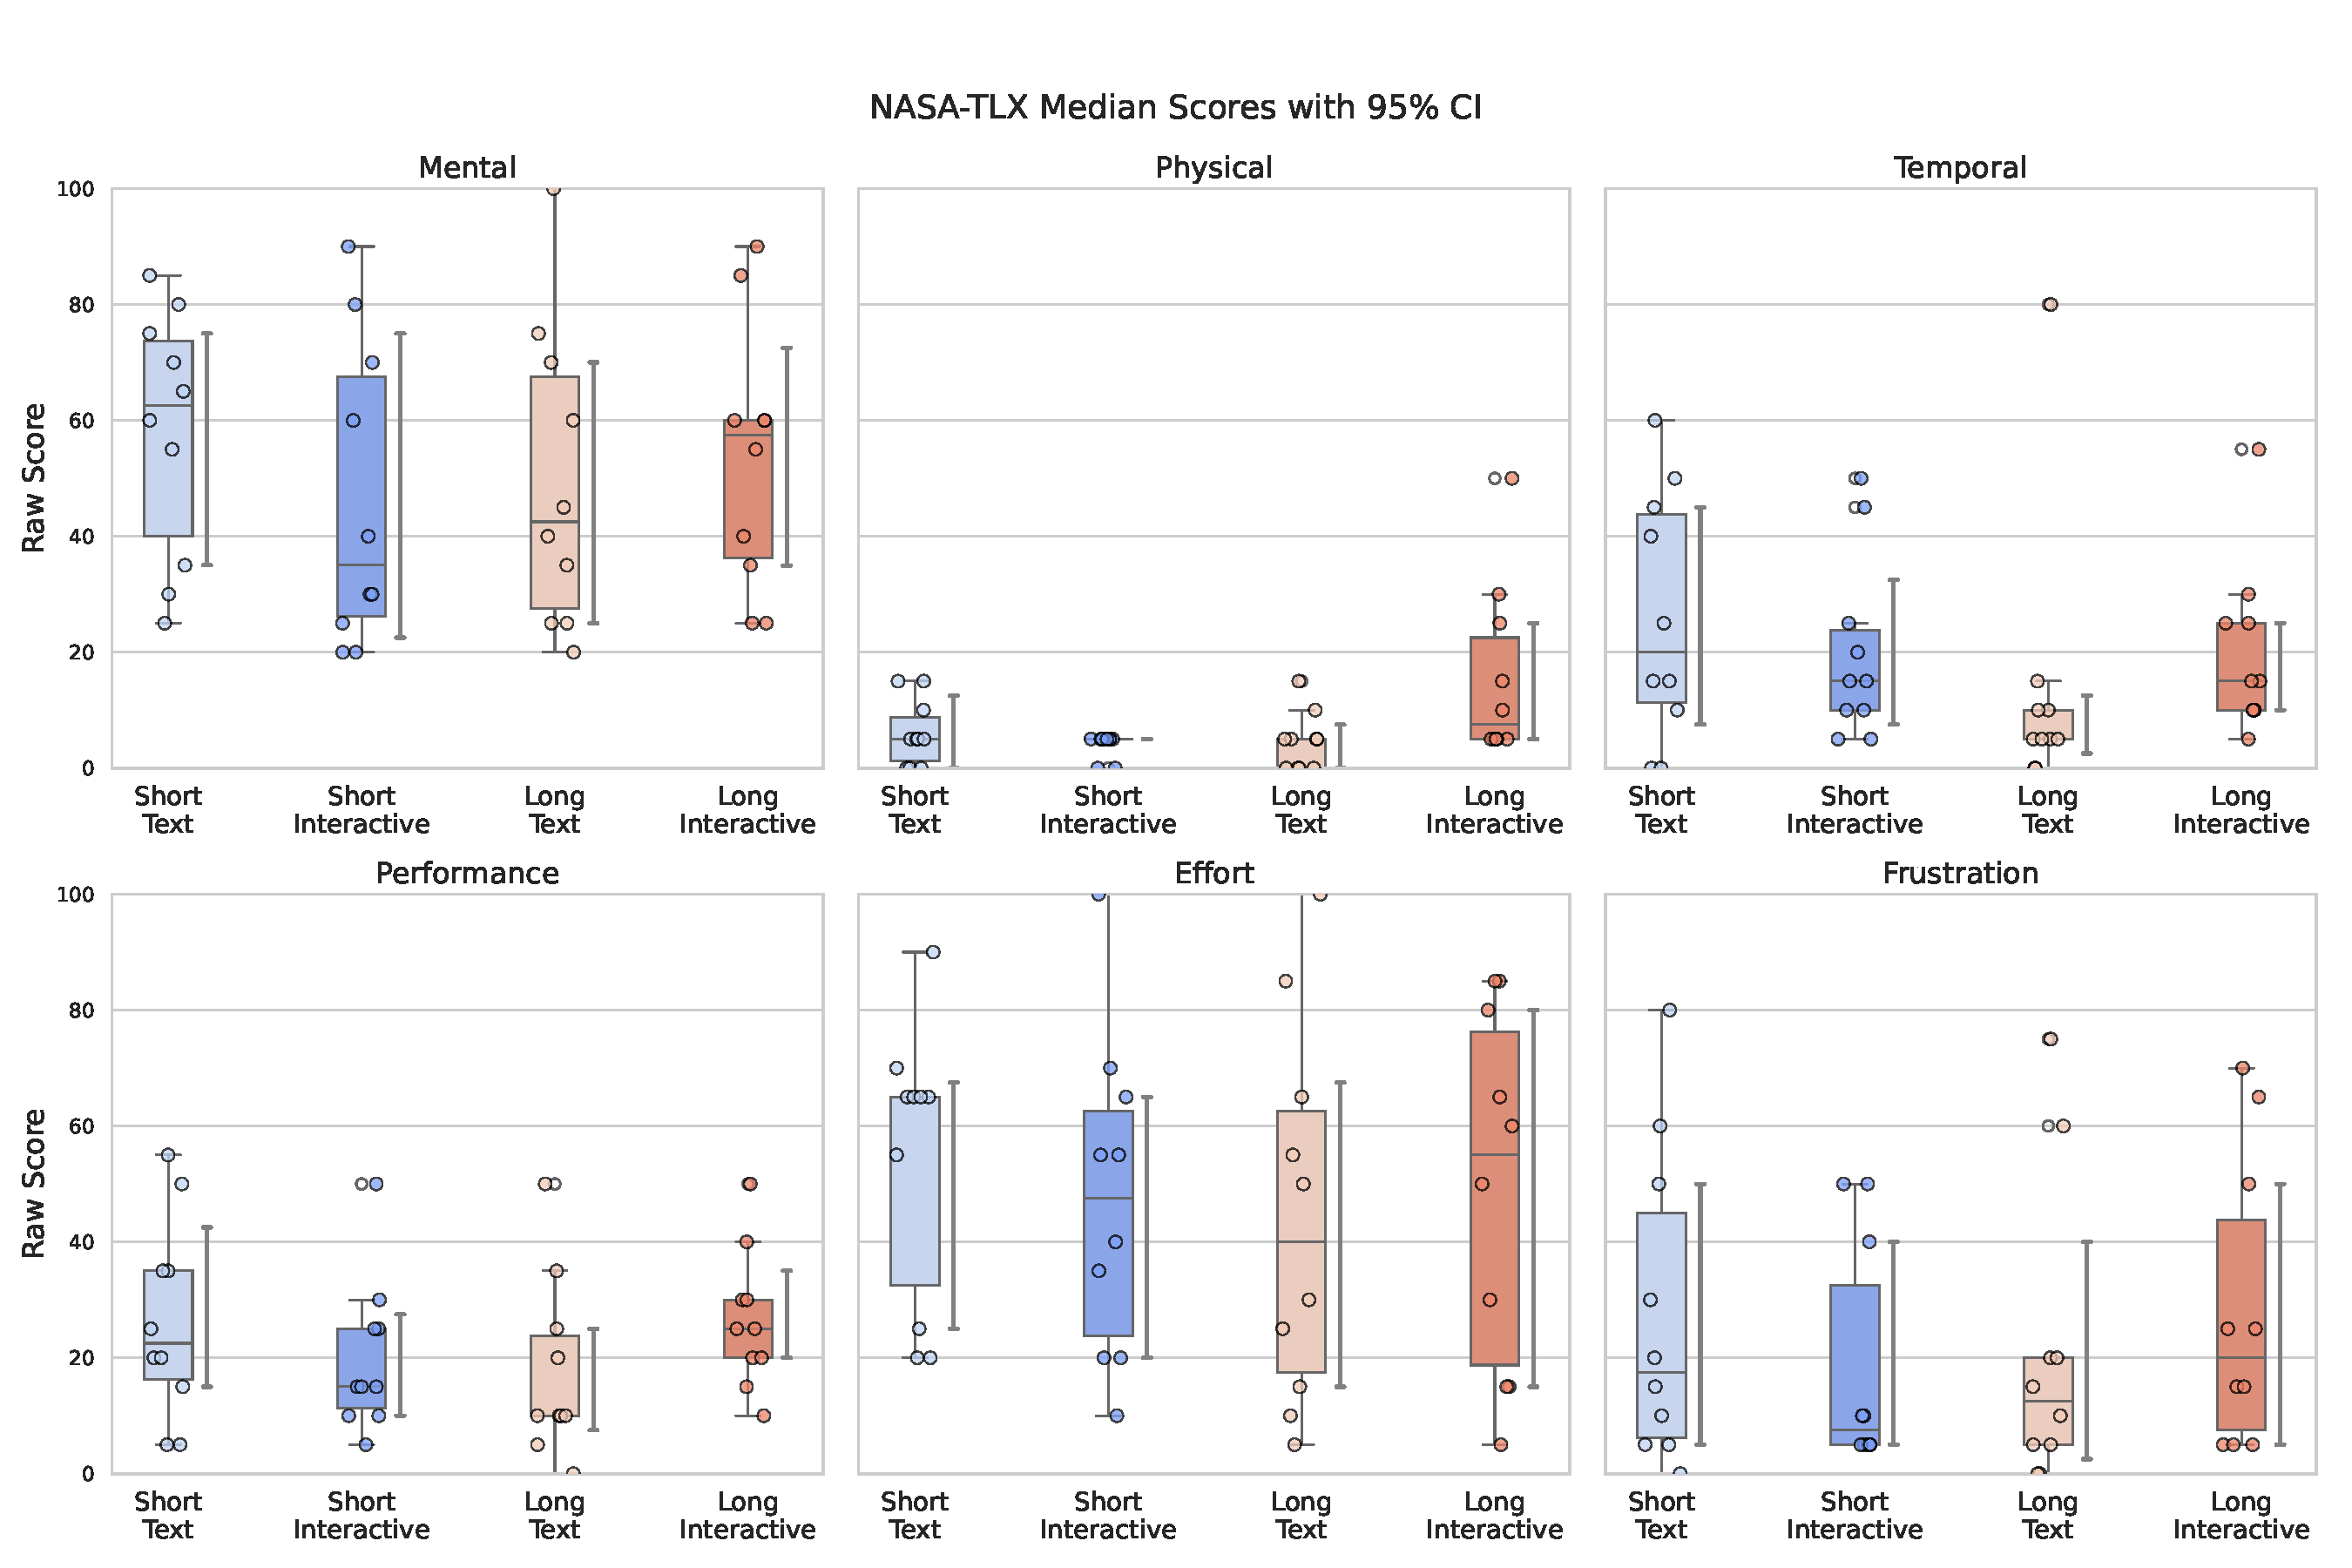
\includegraphics[width=\textwidth]{content/image/cog/nasatlx_final_value_with_CI.pdf}
%     \caption{NASA-TLX Results}
%     \label{fig:nasatlx-with-ci}
% \end{figure}





% Removed text yeard
%% Mental Demand

%\subsubsection{Mental Demand Source: Other Sources}
%We identified four additional sources causing participants' mental demands: \textit{experiment setup}, \textit{number of options}, \textit{QS mechanism}, and \textit{external factors}. 

%$24$ participants mentioned the experiment setup mainly related to understanding and recalling their experience with the options. $6$ participants, all from the long QS, found the number of options added mental demand. $4$ participants cited working with getting familiar with the QS mechanism as a source of mental demand. These are sources related to the study design. $12$ participants mentioned external factors, such as considering the consequences of their results or the challenges decision-makers face. $4$ participants reported an increase and another four a reduction in mental demand due to the interface design. $8$ participants expressed mental demand from justifying their choices and reflecting on their responses, questioning whether their votes truly reflected their preferences or if the amount of credit spent was justified.
% 
%In the first quote, participants felt mental demand focusing on three options, trying to recall specific characteristics to differentiate them. In the second quote, participants considered the societal impact of options, aiming to maximize their effect. This difference highlighted our belief that the organization phase prompted participants to consider a broader range of factors in their decisions. Across both interfaces, participants in the long survey tended towards operational mental demands related to budget management. 

% In addition, we also find that long text interface participants focused on more operational behaviors such as:

% \begin{displayquote}
% So I wanted to be fair.~\bracketellipsis I actually took my calculator out and said~\bracketellipsis  how much would it be if I equally distributed it and then how do I do that? Do I wanna do it all equally or not?

% \noindent \hfill -- S020, long text interface
% \end{displayquote}

% compared to more procedures involving more strategic planning such as:

% \begin{displayquote}
% I wanted to make sure I wanted to give some credit to everything~\bracketellipsis I'm trying to make sure that I had without doing a lot of~\ldots I guess redos is trying to kind of get it right the first time on how I weight things.

% \noindent \hfill -- S032, long two-phase interface
% \end{displayquote}



% IN_T4: Wanting more information on the options~(N=6/40)
% 5. While the numbers seem small, non of this request came from v3. This could explain that participants are already overloaded from the existing the task.